%导言区
\documentclass{report}

\title{SP Final Project Report}
\author{Chao Yang, Xun Liao, ChuYang Xiao}
\date{\today}

\usepackage{graphicx}
\usepackage{subfigure}
\usepackage{caption}
\graphicspath{{latex report/}}

%正文区
\begin{document}

\maketitle

\begin{figure}[htbp]
\section{Question 1}
We first load Observation.nb.mat, which introduces all the variables needed in this section.


\centering
\subfigure[time domain of microphone1]{
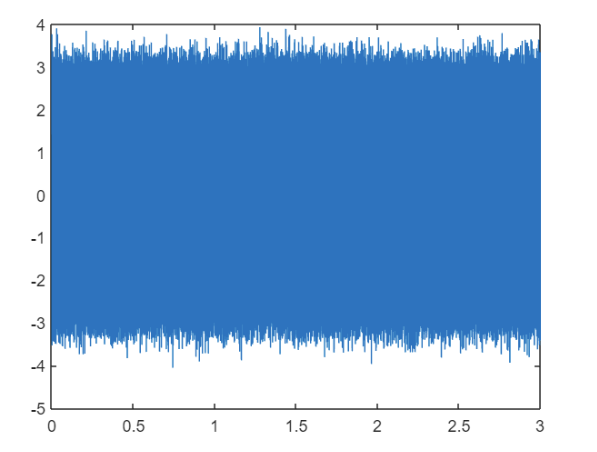
\includegraphics[width=5.5cm]{time domain 1}
%\caption{fig1}
}
\quad
\subfigure[time domain of microphone2]{
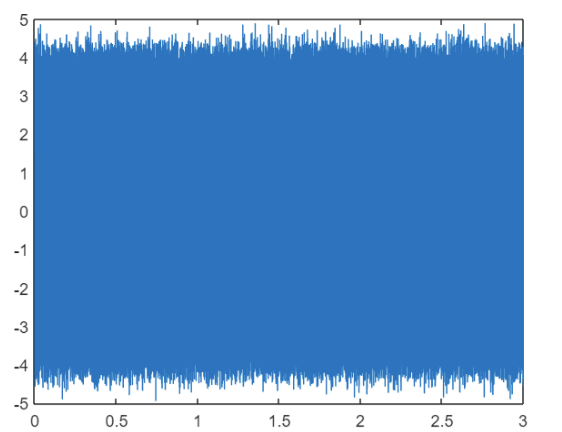
\includegraphics[width=5.5cm]{time domain 2}
}
\quad
\subfigure[time domain of microphone3]{
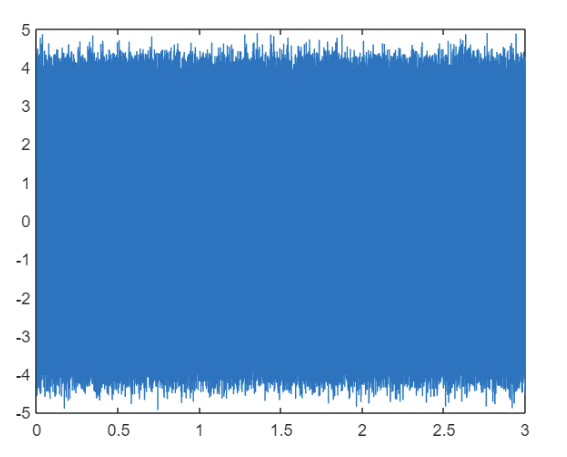
\includegraphics[width=5.5cm]{time domain 3}
}
\quad
\subfigure[time domain of microphone4]{
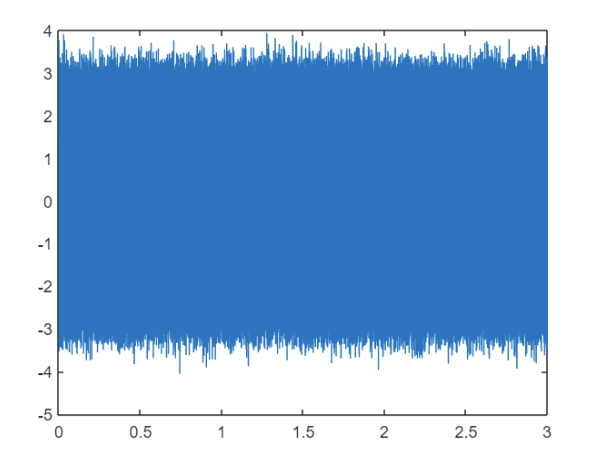
\includegraphics[width=5.5cm]{time domain 4}
}
\caption{time domain}
\end{figure}
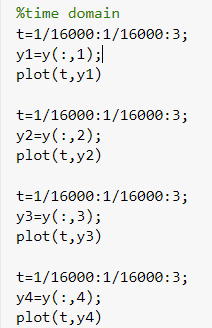
\includegraphics[scale=0.7]{code time domain}
\\Plot the time domain of 4 microphones.
\begin{figure}


\end{figure}



\newpage
\begin{figure}

\centering
\subfigure[frequency domain of microphone1]{
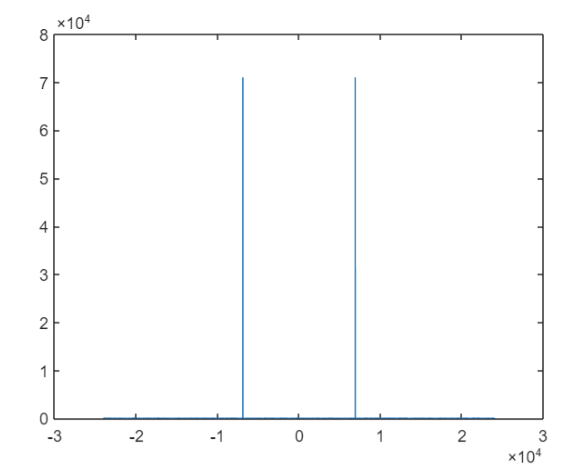
\includegraphics[width=5.5cm]{fre domain 1}
%\caption{fig1}
}
\quad
\subfigure[frequency domain of microphone2]{
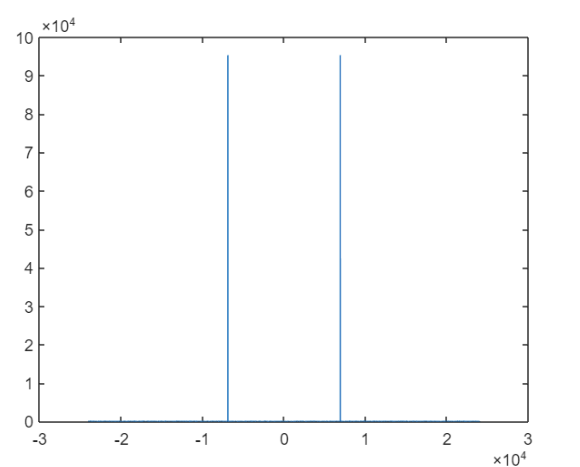
\includegraphics[width=5.5cm]{fre domain 2}
}
\quad
\subfigure[frequency domain of microphone3]{
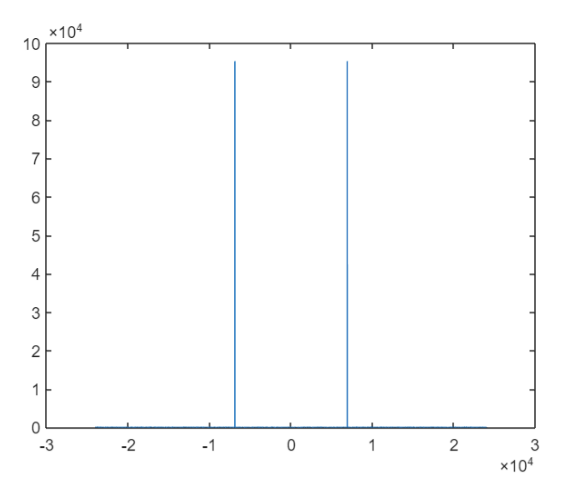
\includegraphics[width=5.5cm]{fre domain 3}
}
\quad
\subfigure[frequency domain of microphone4]{
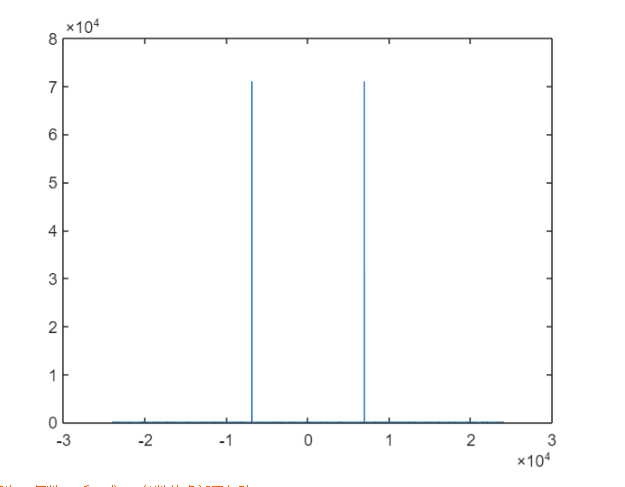
\includegraphics[width=5.5cm]{fre domain 4}
}
\caption{frequency domain}


\end{figure}

\begin{figure}
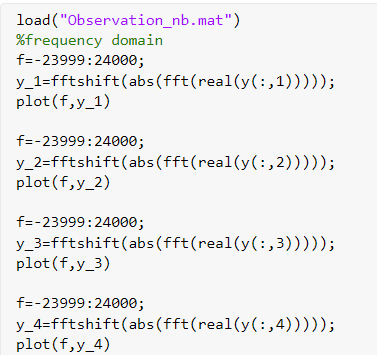
\includegraphics[scale=0.7]{code fre domain}
\\Plot the frequency domain of 4 microphones.
\end{figure}

\begin{figure}
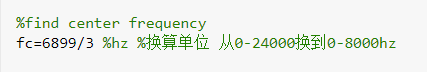
\includegraphics[scale=0.7]{code center fre}
\\Find the center frequency from the figure of frequency domain.
\end{figure}

\begin{figure}
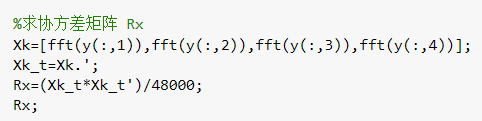
\includegraphics[scale=0.7]{code Rx}
\\Find Rx, according to the fomula$Rx=\frac{1}{N} \cdot \sum_{k=1}^{N}{x[k] \cdot x[k]'}$
\\x[k] is a 4*48000 matrix, x[k]*x[k]' is a 4*4 matrix and N is48000.
\end{figure}

\begin{figure}
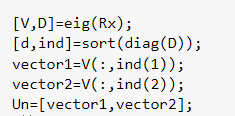
\includegraphics[scale=0.7]{code eigenvector}
\\Find two min eigenvalue's corresponding eigenvectors.
\end{figure}

\begin{figure}
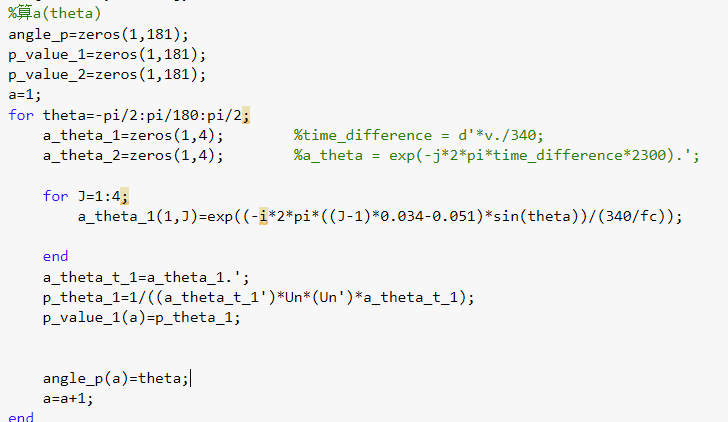
\includegraphics[scale=0.7]{code a(theta)}
\\Find a(theta),according to the formula below.
\end{figure}
\begin{figure}
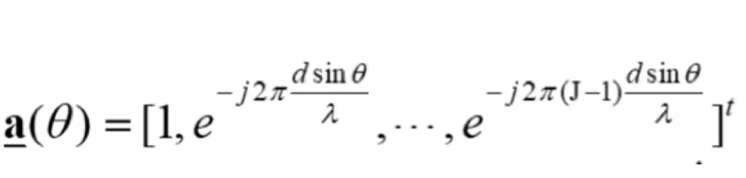
\includegraphics[scale=0.3]{formula1}
\end{figure}



\begin{figure}
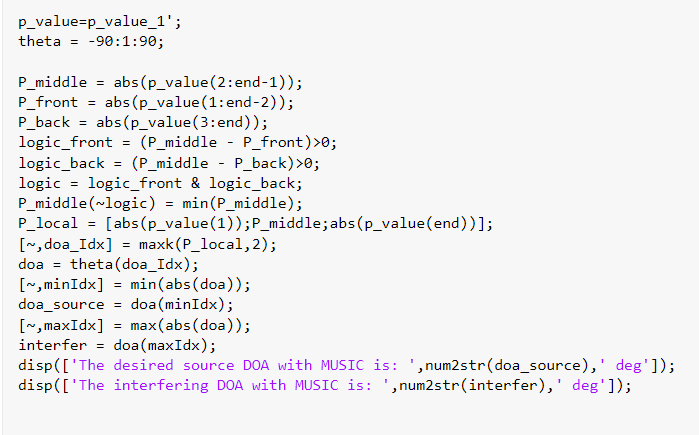
\includegraphics[scale=0.7]{code find direction}
\\Use the provided code to find two directions of both the desired narrowband source signal and the second interfering signal.
\end{figure}


\newpage
\begin{figure}
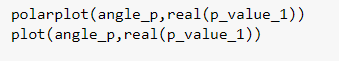
\includegraphics[scale=0.7]{code plot doa and spectrum}
\\Plot the figure of 'doa estimation' and 'pseudo spatial spectrum'.
\end{figure}

\begin{figure}[htbp]
\subfigure[doa] %第一张子图
{
	\begin{minipage}{7cm}
	       %子图居中
	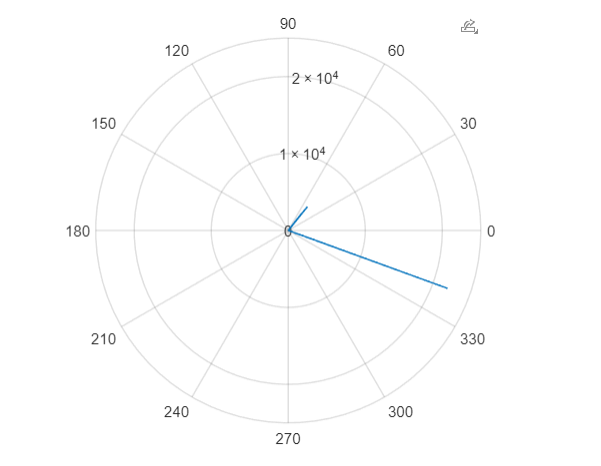
\includegraphics[scale=0.5]{A}   %以pic.jpg的0.5倍大小输出
	\end{minipage}
}
	\subfigure[spectrum] %第二张子图
{
	\begin{minipage}{7cm}
	    %子图居中
	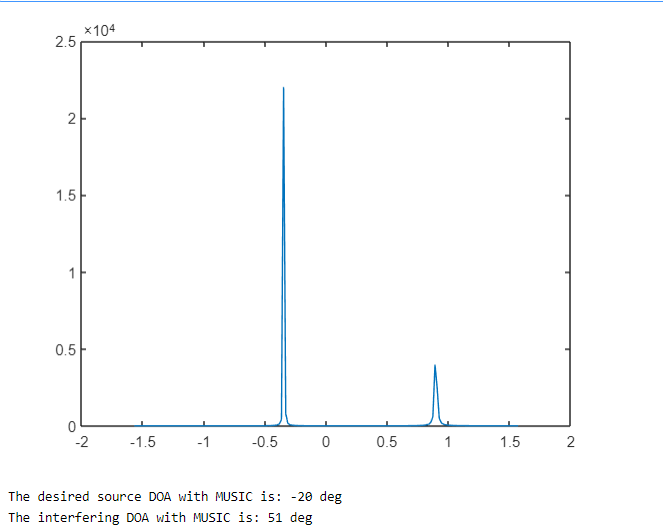
\includegraphics[scale=0.5]{pseudo spatial spectrum}   %以pic.jpg的0.5倍大小输出
	\end{minipage}
}
 
\caption{the second question} %  %大图名称
\label{fig:1}  %图片引用标记
\end{figure}










%\includegraphics[scale=0.5]{doa estimation}
%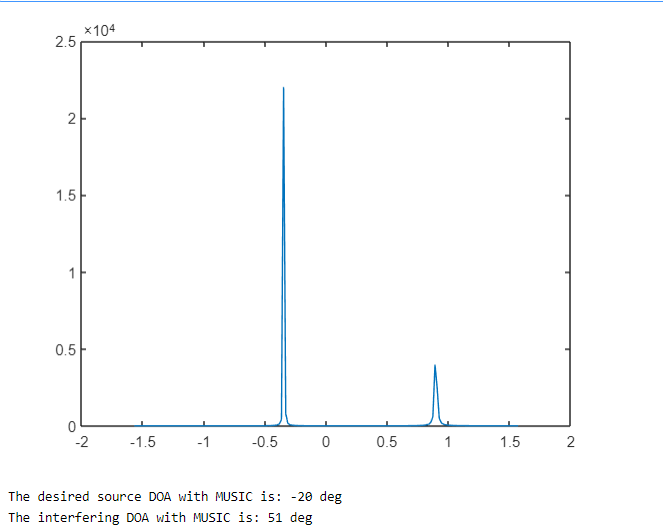
\includegraphics[scale=0.5]{pseudo spatial spectrum}










%\begin{figure}
%\section{Question 1}
%\centering
%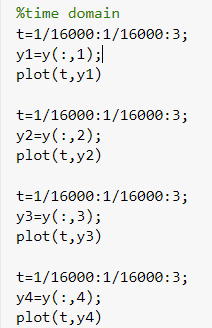
\includegraphics[scale=0.7]{code time domain}
%\end{figure}



   

   

   
%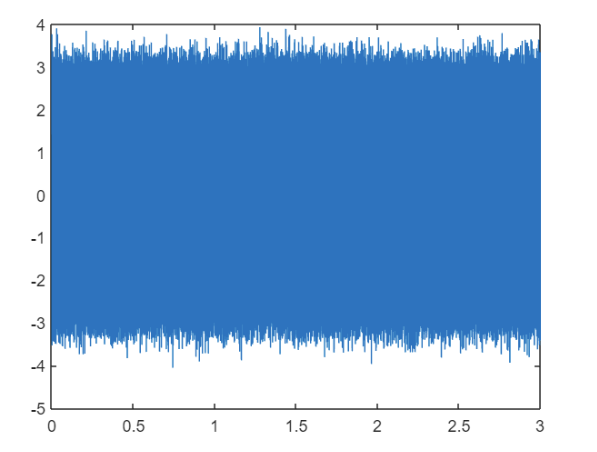
\includegraphics[scale=0.7]{time domain 1}

%	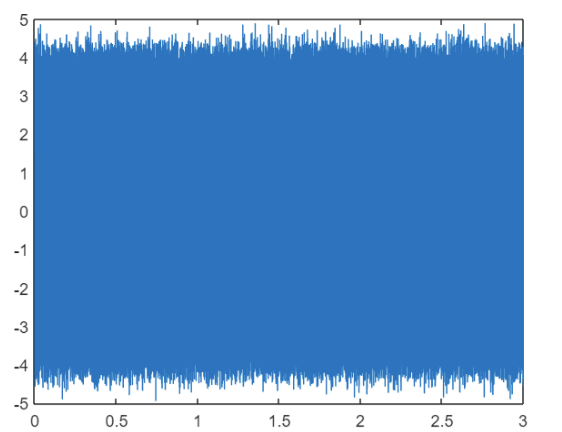
\includegraphics[scale=0.7]{time domain 2}
%	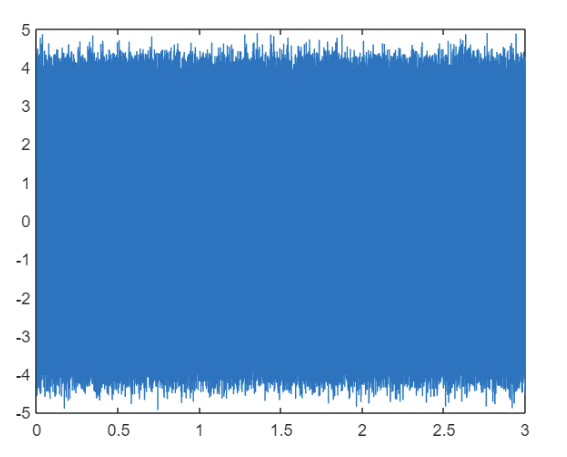
\includegraphics[scale=0.7]{time domain 3}
%	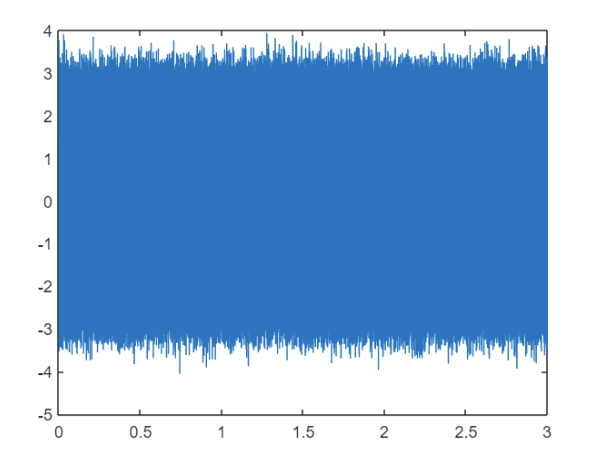
\includegraphics[scale=0.7]{time domain 4}
	
	


\end{document}